\documentclass[../main.tex]{subfiles}

\graphicspath{{../images/}}

\begin{document}
\pagestyle{fancy}
\lhead{Junseo Shin \& Jeremy Smith}
\rhead{Lab Notebook: Fourier Methods}
\chead{9/17/24-9/19/24}
\section{The Fluxgate Magetometer}

% chapter 13
\subsection*{Chapter 13: Understanding the Fluxgate Magnetometer}
\addcontentsline{toc}{subsection}{Chapter 13: Understanding the Fluxgate Magnetometer}
\paragraph{Notes}

\begin{itemize}
    \item Teachspin Fluxgate Magnetometer Module:
    \begin{itemize}
        \item Fluxgate Sensor: 
        \item Double Solenoid: Two electrically separate wires are wound and stored in a tube for the fluxgate sensor to fit in. This is so we can have up to two independently added magnetic fields. 
        \begin{itemize}
            \item Solenoid pitch $= 2.54$ mm, and the expected magnetic field inside the Solenoid is given by
           \begin{align*}
               B_\text{ext} = 2 \mu_0 n i
           \end{align*} 
            where $i$ is the current through a solenoid, $2$ accounts for the doubled layer, and the turn density is
            \begin{align*}
                n = 1 \textrm{ turn} / (\qty{0.00254}{m} = \qty{394}{m^{-1}} 
            \end{align*}
            From this, the magnitude of the external magnetic field given a current $i$ is
            \begin{align*}
                \frac{B_\text{ext}}{i} = 2 \cdot (4 \pi \qty{e-7}{T m / A}) \qty{394}{/m} = \qty{990}{\micro T/A}
            \end{align*}
        \end{itemize}
        \item Modeling Output: Calibrating the Solenoid
        \begin{itemize}
            \item For simple models the 2$f$-component of the field is linear $A = S B_\text{ext}$, but we are actually measuring the magnitude of the spectral component
            \begin{align*}
                M = S \abs{B_\text{ext}}
            \end{align*}
            \item The geometry of the vector components require us to take a phaser sum which gives us the square magnitude of the measured field
            \begin{align*}
                M^s = S^2 \qt[
                    \qt(
                        B_\text{ext} + \frac{A_{para}}{S}
                    )^2 + \qt(
                        \frac{A_{perp}}{S}
                    )^2
                    )
                ] = S^2 \qt[(B_{ext} + a)^2 + b^2]
            \end{align*}
        \end{itemize}
    \end{itemize}
 
\end{itemize}

% fig exp3_1.png and exp3_2.png
\begin{figure}[ht]
    \centering
    \begin{tabular}{cc}
        \includegraphics[width=0.45\linewidth]{exp3_1.png} & \includegraphics[width=0.45\linewidth]{exp3_2.png} \\
        (a) & (b)
    \end{tabular}
    \caption{(a) Fluxgate Magnetometer sensor components and (b) Fluxgate sensor and double solenoid setup}
    \label{fig:exp3_combined}
\end{figure}
In this project we will be learning how to use a fluxgate magnetometer in correspondence with the Fourier analysis done by the SSR770. This allows us to measure even the smallest of magnetic fields. Our understanding is that when displayed on the SSR we will find see the harmonics of the currrent coming out of the fluxgate. With the first fundamental harmonic we will see current of the driving AC coil, but for the second harmonic, we will see the actual readings due to external fields superimposed upon it. This is similar to the AM modulation except instead of program content we have magnetic field strength data.

\paragraph{Experimental Setup}
\begin{itemize}
    \item SR770 Config:
    \begin{itemize}
        \item FREQ: 3.125 kHz to view $2f$ and 12.2 Hz for measurement; Center Freq. 2 kHZ (second harmonic)
        \item MEASure: Spectrum, Flattop Window
        \item Average: 16, Exponential
        \item SOURCE OUT: 1 kHz 1 V 
    \end{itemize}
\end{itemize}

\paragraph{Procedure}
\begin{itemize}
    \item 770: 1 kHz 1 V Sine SOURCE OUT $\to$ Power Audio Amp. module and adjust gain to 6 V (monitor output with splitter to scope)
    \item Power Audio Amp. output $\to$ Fluxgate Primary (AC drive) coil
    \item Secondary (pick-up) coil $\to$ SR770 input
    \item Rotate the sensor to find the maximum signal 
    \item Measure second harmonic $2f$ component of the frequency spectrum
    \item Add 2.5 V DC current (from 33500 B) to Solenoid A and measure the changes in the $2f$ component
    \begin{itemize}
        \item NOTE: Use 50 Ohm Terminator so the measured ouput voltage is exactly the displayed voltage due to the internal 50 Ohm impedence of the 33500B
    \end{itemize}
    \item 770 config change: FREQ SPAN 12.2 Hz
    \item Solenoid A: Replace DC current with AC ($f_A = 5$ Hz 1 V Sine wave from 33500B) and find the $2f \pm f_A$ components
    \item Solenoid B: Add a second AC drive ($f_B = 2.5$ Hz 0.5 V Sine wave from second 33500 B) and measure the four side band frequencies $2f \pm f_A, 2f \pm f_B$
\end{itemize}

\newpage
\paragraph{Observations}
\begin{figure}[ht]
    \centering
    \includegraphics[width=0.5\linewidth]{Magnetometer Data.jpg}
    \caption{Frequency data from the fluxgate magnetometer onto the SR770}
    \label{fig:mag data}
\end{figure}

\begin{figure}[ht]
    \centering
    \begin{tabular}{cc}
        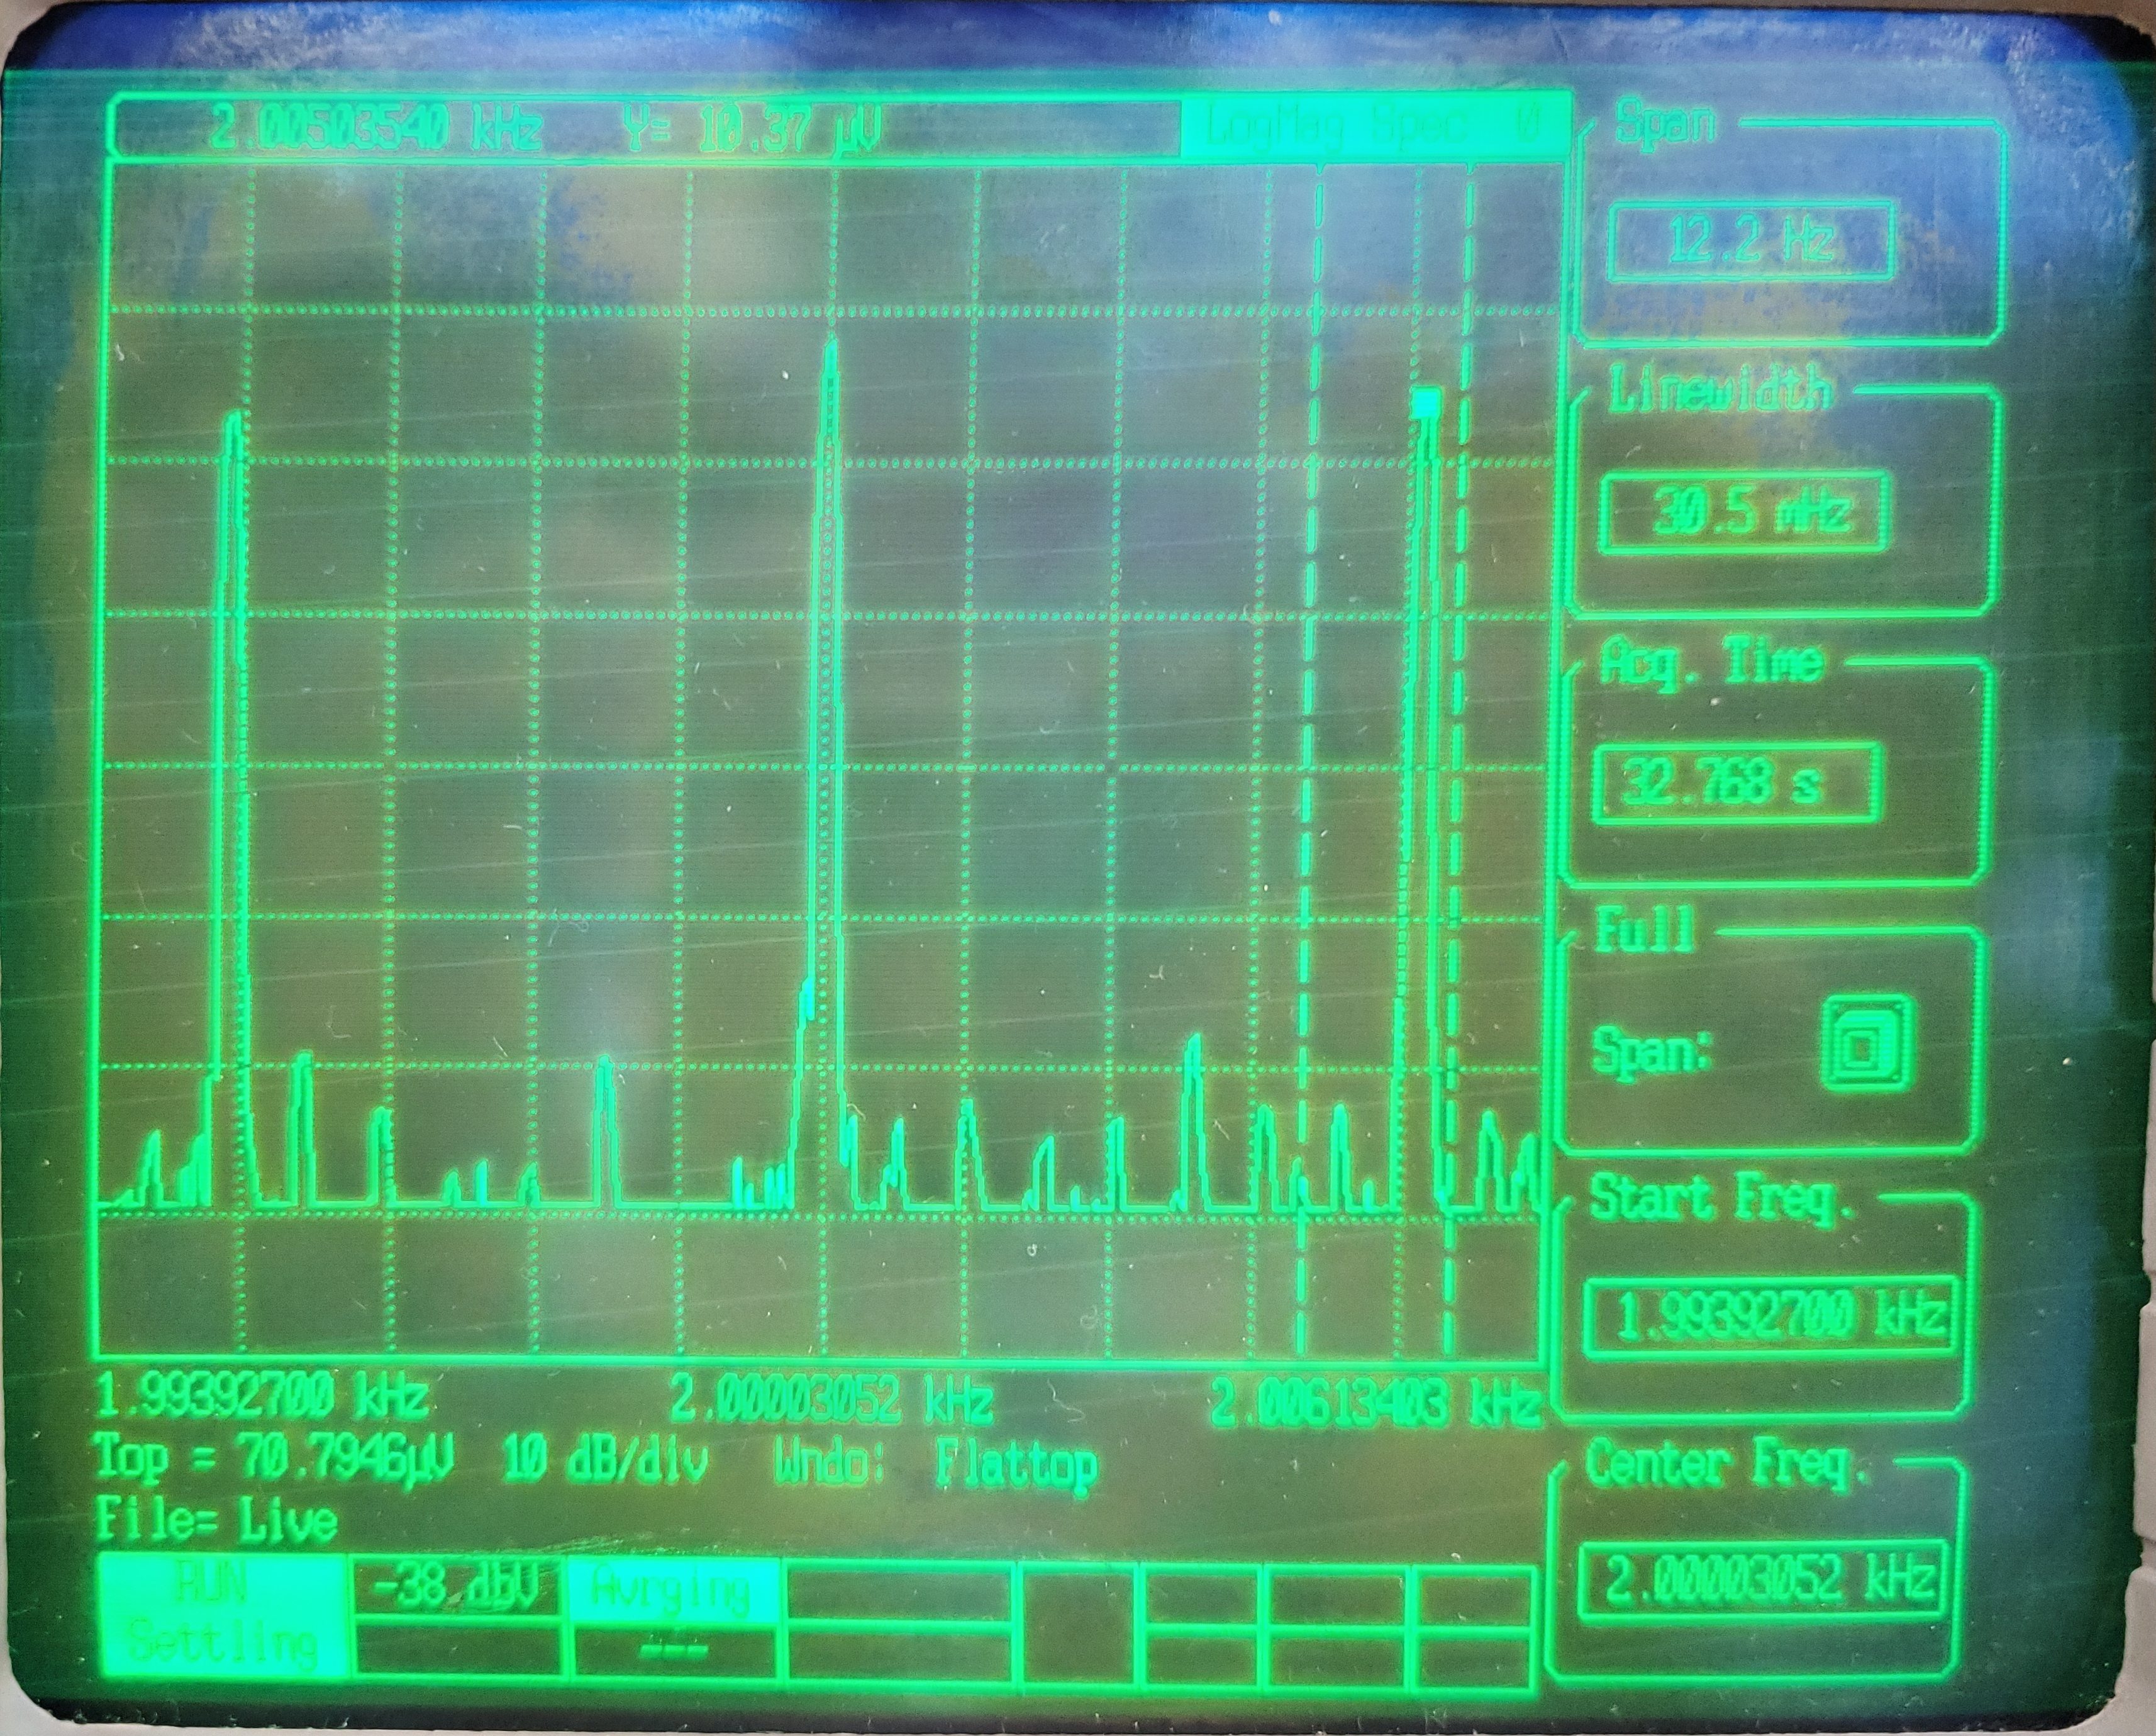
\includegraphics[width=0.45\textwidth]{Fluxdata2.jpg} &
        \includegraphics[width=0.45\textwidth]{fig3.4} \\
        (a) & (b)
    \end{tabular}
    \caption{(a) SR770 view of fluxgate sensor with one external AC magnetic field (b) two external AC magnetic fields applied to double solenoid}
    \label{fig:exp3_2}
\end{figure}
From these we are able to see that the 2nd harmonic can be measured via their Voltage Spectral Density. After calibration we are able to measure the magnetic field that it is detecting. We can then, as in the 2nd image, zoom into the further harmonics to see even finer and finer levels of specificity with the fluxgate. At this small a range of frequency we are able to measure even at the level of $\mu$ Teslas, Able to detect the effects of the earths magnetic field. We even noticed that the nearby NMR machine was able to be seen by our setup.

\end{document} 